\documentclass{article}

\usepackage{mathptmx,fullpage}
\usepackage{amssymb,amsmath,amsthm,mdframed,tikz}
\usetikzlibrary{decorations.pathreplacing}

\newtheorem{thm}{Theorem}
\newtheorem*{dfn}{Definition}
\newtheorem{cor}[thm]{Corollary}
\newtheorem{lem}[thm]{Lemma}
\newtheorem{claim}{Claim}


\newcommand{\ket}[1]{|#1\rangle}
\newcommand{\bra}[1]{\langle#1|}
\newcommand{\braket}[2]{\langle#1|#2\rangle}
\newcommand{\bbC}{\mathbb{C}}
\newcommand{\calH}{\mathcal{H}}

\DeclareMathOperator{\poly}{poly}

\begin{document}

\noindent
\fbox{
	\parbox{\linewidth}{
		\vspace{-.3cm}
{\bf \Large \begin{center}
CS 593/MA 592 - Intro to Quantum Computing \\
Spring 2024 \\
Tuesday, February 27 - Lecture 8.1
\end{center}}
Today's scribe: Nico
	}
}

\vspace{.3cm}

\noindent{\bf Agenda:}
\begin{enumerate}
\item Quantum Simulation
\item The Heisenberg Model
\end{enumerate}
Intended to cover the Ising model, but did not get to it.

\section{Quantum Simulation}

Given a ``reasonable" description of a (discrete) quantum mechanical system, we expect that we can simulate the system on a quantum computer. This expectation comes from the classical case. We can simulate classical mechanical systems on classical computers pretty well.

\vspace{0.5cm}

In the classical setting, we have two main ways to describe dynamical systems:

\vspace{0.5cm}

\noindent\textbf{Newtonian Mechanics: } We have a description of a force vector $\vec{F}$ on space. To simulate time evolution/dynamics, we use Newton's equation $$\frac{d}{dt}\left (m\frac{d\vec{x}}{dt}\right ) = \vec{F}$$ which amounts to solving some differential equation.

\vspace{0.5cm}

\noindent\textbf{Hamiltonian Mechanics: } Instead of a force vector field, we are given a Hamiltonian $\mathcal H$ which is a function on phase space to $\mathbb R$. This yields Hamilton's equations: $$\left \{\begin{matrix}
     \frac{d\vec{q}}{dt} = \frac{\partial \mathcal H}{\partial \vec{p}}  \\
     \frac{d\vec{p}}{dt} = -\frac{\partial \mathcal H}{\partial \vec{q}} 
\end{matrix}\right .$$

In quantum mechanics, we use the quantum version of Hamiltonian mechanics. According to Schr\"odinger, for a quantum mechanical system with state space $V$, the time evolution is controlled by a (quantum) Hamiltonian $\mathcal H$, which is a Hermitian operator $V\to V$, thought of as the \textit{energy observable}. The axioms of quantum mechanics tell us that the Hamiltonian generates the dynamics of a quantum mechanical system via Schr\"odinger's equation: $$i\hslash \frac{\partial}{\partial t}|\psi\rangle = \mathcal H|\psi\rangle$$
Thus, given an explicit description of $\mathcal{H}$, simulating the corresponding quantum mechanical system requires that we (exactly/numerically/approximately according to our goals) solve this differential equation.

In all of these cases, ideally we would like to be able solve these differential equations explicitly by finding exact analytic solutions.  But this is generally not possible even classically (e.g. the three-body problem). So, instead of solving, we try to \textit{simulate} the dynamics using a computer.

The simulation takes in some inputs (initial state, initial time, and accuracy $\delta>0$) and yields an output which is an approximation of the time evolved state after some time $t$ to within $\delta$-accuracy. Classically, this can be done by \textbf{discretizing} using various methods (finite element method, etc.), but quantum mechanically, this is trickier. In fact, we don't really have any better of a way to store quantum states on a classical computer besides just storing each amplitude in the computational basis individually. This makes simulation via discretizing states on a classical computer \textbf{extremely costly}.

Not only is discretizing states costly, but in general discretizing the Hamiltonian $\mathcal H$ is costly as well! Luckily, however, most Hamiltonians encountered in physics are \textit{``local"}, i.e. they are made up of smaller Hamiltonians which only act on a bounded number of particles at a time.

\begin{mdframed}
    Any Hamiltonian $\mathcal H$ may be decomposed in the following way: $$\mathcal H = \sum_{S\subset\{x_1,\dots ,x_n\}}\mathcal H_S$$ where $x_i$ is a qubit, and $\mathcal H_S$ is a Hermitian operator on $S$, extended to all of $\{x_1,\dots ,x_n\}$ by tensoring with the identity.

\vspace{0.5cm}

\noindent{\textbf{Example: }} Let $n = 6$ and let $S = \{x_1,x_2,x_4\}$, then we could let $\mathcal H_S$ be given by: $$\mathcal H_S = X\otimes (X+Z)\otimes Id\otimes Z\otimes Id^{\otimes 2}$$ or $$\mathcal H_S = CNOT \otimes Id\otimes (X-Z)\otimes Id^{\otimes 2}$$
\end{mdframed}

\vspace{0.5cm}

To remedy these issues, Yuri Manin and Richard Feynman proposed that we simulate quantum systems on quantum computers.

\subsection{The Heisenberg Model}

Consider a ``spin chain" comprised of tiny spins or magnets:

\begin{center}
    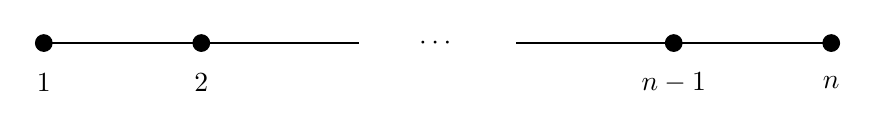
\begin{tikzpicture}
        \filldraw (0,0) circle (3pt);
        \filldraw (2,0) circle (3pt);
        \filldraw (8,0) circle (3pt);
        \filldraw (10,0) circle (3pt);
        \node at (5,0) {$\cdots$};
        \draw (0,0) -- (4,0);
        \draw (6,0) -- (10,0);
        \node at (0,-0.5) {$1$};
        \node at (2,-0.5) {$2$};
        \node at (8,-0.5) {$n-1$};
        \node at (10,-0.5) {$n$};
    \end{tikzpicture}
\end{center}

Each spin can be either up or down or in a superposition of both. We can write $$|\text{up}\rangle = |1\rangle \qquad |\text{down}\rangle = |0\rangle$$ and thus we can say that our spin chain is really comprised of $n$ qubits, and thus the state space of our spin chain is $(\mathbb C^2)^{\otimes n}$.

\vspace{0.5cm}

We imagine the neighboring spins are coupled in a "translation invariant way." We do this by choosing coupling constants $(J_x,J_y,J_z)\in \mathbb R^3$ and defining $$\mathcal H_{\text{int}} = -\sum_{j=1}^{n-1} J_x X_j X_{j+1} + J_y Y_j Y_{j+1} + J_z Z_j Z_{j+1}$$ where $U_jU_{j+1}$ means $Id^{\otimes j-1}\otimes U\otimes U \otimes Id^{\otimes n-j-1}$.

\vspace{0.5cm}

We also may have an external magnetic field affecting our chain, say in the $z$-direction, described by $$\mathcal H_{\text{ext}} = -\sum_{j=1}^n hZ_j,\qquad h\in \mathbb R$$ Then we may define $$\mathcal H = \mathcal H_{\text{int}} + \mathcal{H}_{\text{ext}}$$

This is the \textit{Heisenberg model} (for an (anti)ferromagnetic spin chain). As usual, the eigenvalues of $\mathcal H$ are the possible energy levels for our quantum ``magnet" (which may not be a magnet at all!).

\vspace{0.5cm}

Some natural questions may arise: 
\begin{itemize}
    \item What are the energy levels for a given tuple of coupling constants?
    \item What is the lowest energy level (aka the ground state)?
    \item What about phase transitions?
\end{itemize}

We can get an intuition for the energy states by looking at a specific example:

\vspace{0.5cm}

Suppose $J=J_x = J_y=J_z$, then we call the resulting spin chain the \textbf{XXX chain}. When $J>0$, then low energy configurations are ``ferromagnetic" meaning the spins are aligned. I.e. our states might look like $\alpha |0\cdots 0\rangle + \beta|1\cdots 1\rangle$. When $J<0$, the configurations are ``anti-ferromagnetic" which means that the neighboring spins are opposite on average. You should be thinking of states that look like $\alpha |10\cdots 10\rangle + \beta|01\cdots 01\rangle$ (if $n$ is even). For a more thorough analysis of this stuff, you might look up the phrase "Bethe ansatz."


\subsection{Back to Simulation}

Assume that we have a Hamiltonian on $(\mathbb C^2)^{\otimes n}$ $$\mathcal H = \sum_{k=1}^L \mathcal H_k$$ where $L$ is a polynomial in $n$ and each $\mathcal H_k$ is \textit{$c$-local} meaning it is supported on at most $c$ of the $n$ qubits. $\mathcal H$ is called a \textit{$c$-local Hamiltonian on $n$ qubits}.

\vspace{0.5cm}

We would like to simulate the dynamics given by $\mathcal H$. I.e. given a state $|\psi\rangle$, a time $t$, and an accuracy $\delta>0$, we want to use a quantum computer to prepare a state $|\phi\rangle$ which ``approximates the time evolution," i.e. is close to the true time evolution $e^{it\mathcal{H}}\ket{\psi}$ in that $$\left |\langle \phi | e^{it\mathcal H}|\psi\rangle \right |^2 \geq 1-\delta.$$ Moreover, we'd like to do all of this as efficiently as possible in terms of the parameter $n$, $t$, and $\delta$.

The main trick to accomplishing this is sometimes called ``Trotterizing."

\begin{lem}[Trotter Formula]
    For $A,B$ Hermitian, $t\in \mathbb R$, $$\lim_{n\to \infty}\left (\exp(iAt/n)\exp(iBt/n)\right )^n = \exp(i(A+B)t)$$
\end{lem}

\begin{proof}
    \begin{align*}
        \lim_{n\to \infty}\left (\exp(iAt/n)\exp(iBt/n)\right )^n &= \lim_{n\to \infty}\left [ \left (I+\frac{iAt}{n} + O(1/n^2)\right )\left (I+\frac{iBt}{n} + O(1/n^2)\right )\right ]^n\\
        &= \lim_{n\to\infty}\left [I+\frac{i(A+B)t}{n} + O(1/n^2)\right ]^n\\
        &= \lim_{n\to\infty}\left [\sum_{k=0}^n \begin{pmatrix} n\\k \end{pmatrix} \frac{1}{n^k} \big (i(A+B)t\big )^k + O(1/n)\right ]\\
    \end{align*}

The last equality comes from using the Binomial theorem.

Note that $$\begin{pmatrix}
    n\\k
\end{pmatrix} = \frac{1+O(1/n)}{k!}$$ so

    \begin{align*}
        \lim_{n\to \infty}\left (\exp(iAt/n)\exp(iBt/n)\right )^n&= \lim_{n\to\infty} \left [\sum_{k=0}^n \frac{1+O(1/n)}{k!} \big (i(A+B)t\big )^k + O(1/n)\right ]\\
        &= \sum_{k\geq 0} \frac{1}{k!}\big (i(A+B)t\big )^k\\
        &= \exp(i(A+B)t)
    \end{align*}
\end{proof}

\begin{claim}
    Fix $c\in \mathbb N$. Given a $c$-local Hamiltonian on $n$ qubits $$\mathcal H = \sum_{k=1}^L \mathcal H_k$$, a state $|\psi\rangle$ and an accuracy $\delta>0$, there is a quantum algorithm to prepare a state $|\phi\rangle$ such that $$\left |\langle \phi |e^{it\mathcal H}|\psi\rangle \right |^2 \geq 1-\delta.$$
Moreover, the algorithm runs in time $O(\poly(1/\delta),t,n)$.
\end{claim}

\begin{proof}[Proof Sketch]
    Since $c$ is fixed, we might as well assume that our gate set includes \emph{all} $c$-ary gates.  Thus, we can assume that we can implement arbitrary $c$-ary gates in one unit of time. In particular, for all $s$, it takes only one unit of time to implement $\exp(is\mathcal H_k)$. Pick $s$ appropriately (given $t$ and $\delta$) and let $U$ be the following circuit, which we describe only schematically:

    \begin{center}
        \begin{tikzpicture}
            \draw (0,-2) rectangle (2,2);
            \draw (3,-2) rectangle (5,2);
            \draw (8,-2) rectangle (10,2);
            \draw (-1,1.75) -- (0,1.75);
            \draw (-1,-1.75) -- (0,-1.75);
            \draw (2,1.75) -- (3,1.75);
            \draw (2,-1.75) -- (3,-1.75);
            \draw (5,1.75) -- (6,1.75);
            \draw (5,-1.75) -- (6,-1.75);
            \draw (7,1.75) -- (8,1.75);
            \draw (7,-1.75) -- (8,-1.75);
            \draw (10,1.75) -- (11,1.75);
            \draw (10,-1.75) -- (11,-1.75);
            \node at (-0.5,0.2) {$\vdots$};
            \node at (2.5,0.2) {$\vdots$};
            \node at (5.5,0.2) {$\vdots$};
            \node at (7.5,0.2) {$\vdots$};
            \node at (10.5,0.2) {$\vdots$};
            \node at (6.5,0) {$\cdots$};
            \draw [decorate,decoration={brace,amplitude=5pt}] (-1.5,-2) -- (-1.5,2) node[midway,xshift = -0.5cm]{$n$};
            \node at (1,0) {\Large{$e^{is\mathcal H_1}$}};
            \node at (4,0) {\Large{$e^{is\mathcal H_2}$}};
            \node at (9,0) {\Large{$e^{is\mathcal H_L}$}};
        \end{tikzpicture}
    \end{center}
This is ``schematic" in the sense that each ``gate" here is really a subcircuit that should consist of a single $c$-ary gate on an appropriate choice of $c$ of the $n$ qubits, according to $\mathcal{H}_i$.

    It is straightforward to verify that $$\left \Vert \exp(it\mathcal H) - U^{\lceil t/s\rceil}\right \Vert <\delta.$$
This implies what we want.
\end{proof}


\end{document}